\documentclass[aspectratio=169, 11pt]{beamer}

\usetheme[progressbar=frametitle, numbering=fraction]{metropolis}
\usepackage[T1]{fontenc}
\usepackage[english]{babel}
\usepackage{amsmath}
\usepackage{siunitx}
\usepackage{booktabs}
\usepackage{csquotes}
\usepackage{tikz}
\usetikzlibrary{arrows.meta, positioning}
\usepackage[backend=biber, style=numeric-comp, sorting=none, maxbibnames=3, giveninits=true, doi=false, isbn=false, url=false]{biblatex}
\addbibresource{references.bib}
\renewcommand*{\bibfont}{\scriptsize}
\graphicspath{{figures/}}

\definecolor{cu}{HTML}{EB6834}
\definecolor{zn}{HTML}{2A78D6}
\setbeamercolor{alerted text}{fg=cu!80!black}

\newcommand{\Cu}{\mathrm{Cu}}
\newcommand{\Zn}{\mathrm{Zn}}
\newcommand{\Tc}{T_\mathrm{c}}

\title{Order--disorder transition of \texorpdfstring{$\beta$}{beta}-brass (CuZn)}
\subtitle{Metropolis Monte Carlo on a rigid lattice}
\author{Tony Pansera and Noé Fourniol}
\institute{CentraleSupélec --- Modélisation et simulation numérique}
\titlegraphic{\hfill
\includegraphics[height=1.1cm]{logo_centralesupelec.png}}
\date{November 2026}

\begin{document}

\maketitle

% ---------------------------------------------------------------------
\begin{frame}{The question}
  \begin{columns}[c]
    \begin{column}{0.48\textwidth}
      \begin{itemize}
        \item $\beta$-brass: CuZn, 50\,\% Zn, bcc lattice
        \item Low $T$: \alert{ordered} B2, Cu on corners ($\alpha$), Zn on centres ($\beta$)
        \item High $T$: Cu and Zn \alert{mixed} at random
        \item Transition at $\Tc \approx \SI{740}{K}$~\cite{NixShockley1938,Massalski1990}
      \end{itemize}
      \medskip
      \textbf{Goal:} find $\Tc$ and see how order disappears, with our own Monte Carlo code
    \end{column}
    \begin{column}{0.5\textwidth}
      \centering
      \scalebox{0.85}{% B2 (CsCl) cell of CuZn, used by report.tex and slides.tex (needs tikz).
% Oblique projection: x to the right, y into the page, z up.
\definecolor{cu}{HTML}{EB6834}
\definecolor{zn}{HTML}{2A78D6}
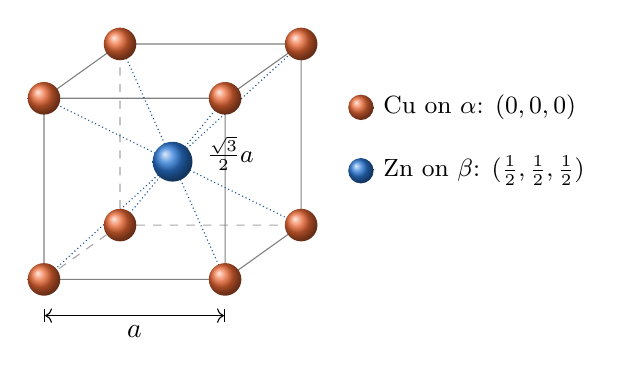
\begin{tikzpicture}[x={(1cm,0cm)}, y={(0.42cm,0.3cm)}, z={(0cm,1cm)}, scale=2.3, line join=round]
  % cube edges: the three edges of the back-bottom-left corner are hidden
  \draw[gray!70, dashed, thin] (0,1,0) -- (0,0,0)  (0,1,0) -- (1,1,0)  (0,1,0) -- (0,1,1);
  \draw[gray, thin] (0,0,0) -- (1,0,0) -- (1,0,1) -- (0,0,1) -- cycle
                    (1,0,0) -- (1,1,0) -- (1,1,1) -- (1,0,1)
                    (0,0,1) -- (0,1,1) -- (1,1,1);
  % the 8 first-neighbour bonds of the centre site
  \foreach \x in {0,1} \foreach \y in {0,1} \foreach \z in {0,1}
    \draw[zn!70!black, densely dotted] (0.5,0.5,0.5) -- (\x,\y,\z);
  % atoms, from the back to the front
  \foreach \x/\z in {0/0,1/0,0/1,1/1} \shade[ball color=cu] (\x,1,\z) circle (0.9mm);
  \shade[ball color=zn] (0.5,0.5,0.5) circle (1.1mm);
  \foreach \x/\z in {0/0,1/0,0/1,1/1} \shade[ball color=cu] (\x,0,\z) circle (0.9mm);
  % distances: a between corners (2nd neighbours), sqrt(3)a/2 corner-centre (1st neighbours)
  \draw[|<->|, thin] (0,0,-0.2) -- (1,0,-0.2) node[midway, below] {$a$};
  \node[font=\small, anchor=west] at (0.74,0.25,0.62) {$\frac{\sqrt{3}}{2}a$};
  % key
  \shade[ball color=cu] (1.75,0,0.95) circle (0.7mm);
  \node[anchor=west, font=\small] at (1.82,0,0.95) {Cu on $\alpha$: $(0,0,0)$};
  \shade[ball color=zn] (1.75,0,0.6) circle (0.7mm);
  \node[anchor=west, font=\small] at (1.82,0,0.6) {Zn on $\beta$: $(\frac12,\frac12,\frac12)$};
\end{tikzpicture}
}
    \end{column}
  \end{columns}
\end{frame}

% ---------------------------------------------------------------------
\begin{frame}{Model: rigid lattice + pair energies}
  \begin{columns}[T]
    \begin{column}{0.5\textwidth}
      \begin{itemize}
        \item Box of $6\times6\times6$ cells: \alert{432 sites}, periodic boundaries
        \item Atoms never leave their site: only \alert{who sits where} changes
        \item Energy = sum over pairs
          \[ E = \sum_{\text{1st}} J_{\sigma_i\sigma_j} + \sum_{\text{2nd}} I_{\sigma_i\sigma_j} \]
        \item 8 first neighbours (other sublattice), 6 second neighbours (same sublattice)
      \end{itemize}
    \end{column}
    \begin{column}{0.46\textwidth}
      \centering
      \small
      \begin{tabular}{lccc}
        \toprule
        eV & Cu--Cu & Zn--Zn & Cu--Zn \\
        \midrule
        $J$ (1st) & $-0.873$ & $-0.338$ & $-0.621$ \\
        $I$ (2nd) & $0$ & $0$ & $+0.005$ \\
        \bottomrule
      \end{tabular}

      \bigskip
      \begin{itemize}
        \item 1st shell prefers \alert{Cu--Zn} pairs
        \item 2nd shell prefers \alert{same-species} pairs
        \item[$\Rightarrow$] both favour B2
      \end{itemize}
    \end{column}
  \end{columns}
\end{frame}

% ---------------------------------------------------------------------
\begin{frame}{Monte Carlo step}
  \centering
  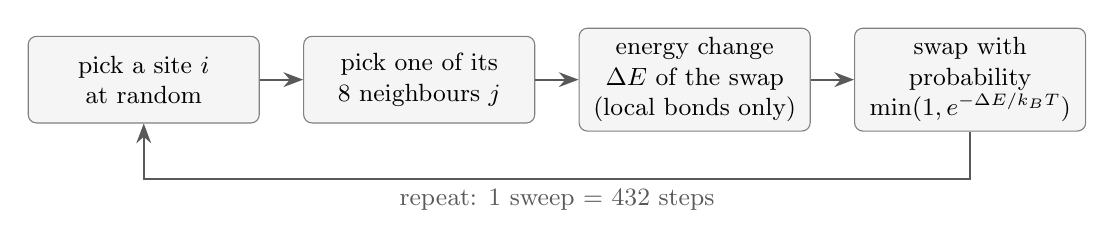
\begin{tikzpicture}[
      box/.style={draw=gray, rounded corners=3pt, fill=gray!8, align=center, minimum height=1.1cm, text width=2.7cm, font=\small},
      arr/.style={-{Stealth[length=2.5mm]}, thick, gray!70!black},
      node distance=0.55cm]
    \node[box] (pick) {pick a site $i$\\at random};
    \node[box, right=of pick] (nb) {pick one of its\\8 neighbours $j$};
    \node[box, right=of nb] (de) {energy change\\$\Delta E$ of the swap\\(local bonds only)};
    \node[box, right=of de] (acc) {swap with\\probability\\$\min(1, e^{-\Delta E/k_BT})$};
    \draw[arr] (pick) -- (nb);
    \draw[arr] (nb) -- (de);
    \draw[arr] (de) -- (acc);
    \draw[arr] (acc.south) -- ++(0,-0.6) -| node[pos=0.25, below, font=\small] {repeat: 1 sweep = 432 steps} (pick.south);
  \end{tikzpicture}

  \vspace{0.6cm}
  \begin{itemize}
    \item \alert{Swaps} keep 216 Cu + 216 Zn (Kawasaki dynamics~\cite{Kawasaki1966}), Metropolis rule~\cite{Metropolis1953}
    \item $\Delta E$ uses 26 bonds instead of 3024: \SI{7}{\micro s} per step in Python
  \end{itemize}
\end{frame}

% ---------------------------------------------------------------------
\begin{frame}{What we measure}
  \begin{itemize}
    \item \alert{Long-range order} (do Cu atoms prefer sublattice $\alpha$?)
      \[ \eta = \frac{N_\Cu^{(\alpha)}-N_\Cu^{(\beta)}}{N_\Cu^{(\alpha)}+N_\Cu^{(\beta)}}
         \quad\begin{cases} 1 & \text{perfect B2}\\ 0 & \text{random}\end{cases}
         \qquad\text{we average } |\eta| \]
    \item \alert{Short-range order} (Cowley~\cite{Cowley1950}): are the neighbours of a Cu more often Zn than at random?
      \[ \alpha_n = 1 - \frac{p_n(\Zn\,|\,\Cu)}{1/2}\qquad \text{B2: } \alpha_1=-1,\ \alpha_2=+1 \qquad \text{random: } 0\]
    \item \alert{Fluctuations} peak at the transition:
      heat capacity $C \propto \langle E^2\rangle - \langle E\rangle^2$,\;
      susceptibility $\chi \propto \langle \eta^2\rangle - \langle |\eta|\rangle^2$
  \end{itemize}
\end{frame}

% ---------------------------------------------------------------------
\begin{frame}{Is the code right?}
  \centering
  \small
  \begin{tabular}{lll}
    \toprule
    Test & Expected & Obtained \\
    \midrule
    Neighbour tables (8 + 6, symmetric) & yes & yes \\
    Perfect B2: $E/N$ & $4J_{\Cu\Zn} = -2.484$ eV & $-2.4840$ eV \\
    Perfect B2: $\eta$, $\alpha_1$, $\alpha_2$ & $1, -1, +1$ & $1, -1, +1$ \\
    Random lattices: $\alpha_1$, $\alpha_2$ & 0, 0 & $-0.002$, $-0.004$ \\
    Random lattices: $\langle|\eta|\rangle$ & $0.038$ (finite size) & $0.038$ \\
    Energy updated step by step vs recomputed & 0 & \SI{4e-12}{eV} \\
    \bottomrule
  \end{tabular}

  \bigskip
  \begin{itemize}
    \item \alert{Cohesive energy} at \SI{0}{K}: \SI{2.484}{eV/atom}
    \item Same model for pure Cu and Zn: 3.49 and 1.35 eV/atom = experimental values~\cite{Kittel2005}
  \end{itemize}
\end{frame}

% ---------------------------------------------------------------------
\begin{frame}{How long before equilibrium?}
  \centering
  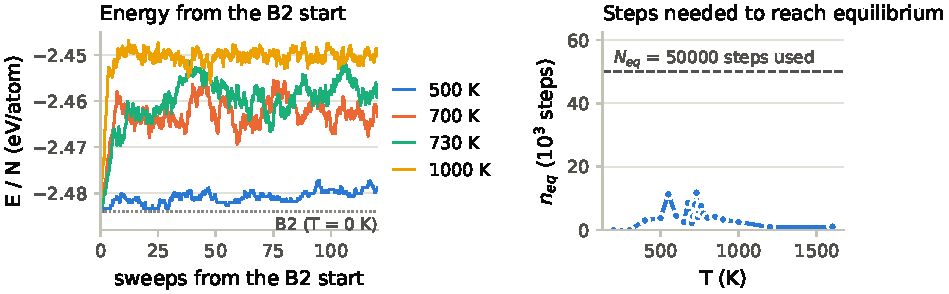
\includegraphics[width=\textwidth]{equilibration.pdf}

  \begin{itemize}
    \item Every run starts from perfect B2 and must \enquote{forget} it
    \item Slowest: about \num{12000} steps $\Rightarrow$ we discard \alert{\num{50000} steps}, then measure \alert{4000 sweeps}
  \end{itemize}
\end{frame}

% ---------------------------------------------------------------------
\begin{frame}{What the crystal looks like}
  \centering
  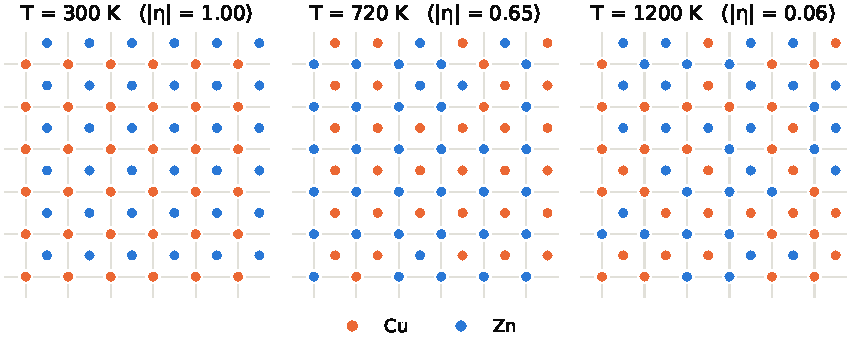
\includegraphics[width=\textwidth]{snapshots.pdf}

  \small One layer of the box: $\alpha$ sites on the grid nodes, $\beta$ sites in the squares.
\end{frame}

% ---------------------------------------------------------------------
\begin{frame}{Energy and heat capacity}
  \centering
  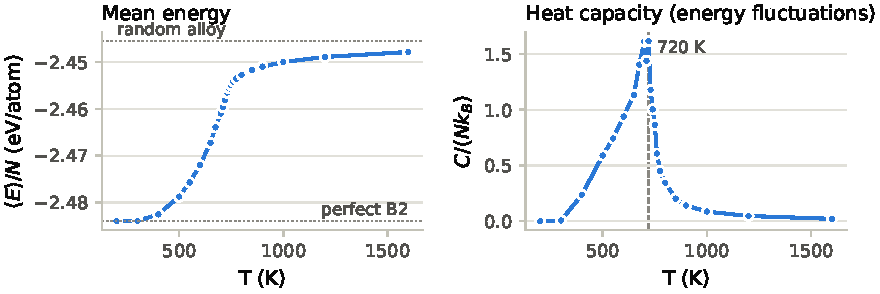
\includegraphics[width=\textwidth]{energy_heat.pdf}

  \begin{itemize}
    \item Energy rises steeply between 600 and \SI{800}{K}
    \item Heat capacity peak at \alert{\SI{720}{K}} (flat top 700--720 K)
  \end{itemize}
\end{frame}

% ---------------------------------------------------------------------
\begin{frame}{Long-range order}
  \centering
  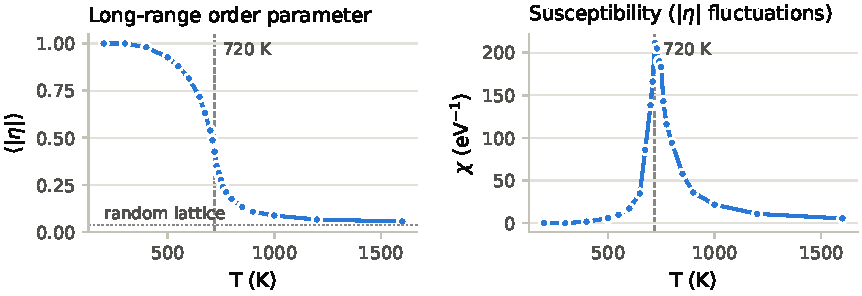
\includegraphics[width=\textwidth]{order_chi.pdf}

  \begin{itemize}
    \item $\langle|\eta|\rangle$ drops fastest at \alert{\SI{720}{K}}, susceptibility peak at \alert{\SI{720}{K}}
    \item Small box: drop is rounded, $|\eta|$ never below the random value 0.04
  \end{itemize}
\end{frame}

% ---------------------------------------------------------------------
\begin{frame}{Near \texorpdfstring{$\Tc$}{Tc} the system hesitates}
  \centering
  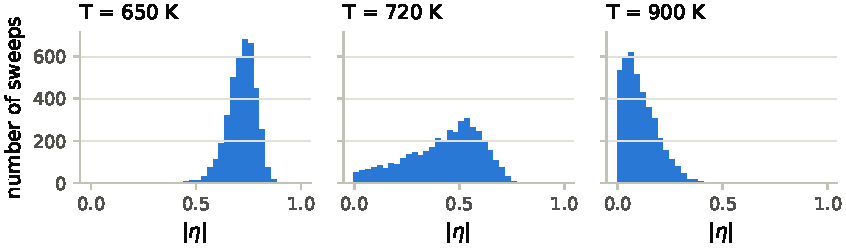
\includegraphics[width=\textwidth]{eta_hist.pdf}

  \begin{itemize}
    \item Below: always ordered \quad Above: always disordered
    \item Near $\Tc$: goes back and forth $\Rightarrow$ \alert{large fluctuations} $\Rightarrow$ peaks of $C$ and $\chi$
  \end{itemize}
\end{frame}

% ---------------------------------------------------------------------
\begin{frame}{Short-range order survives above \texorpdfstring{$\Tc$}{Tc}}
  \centering
  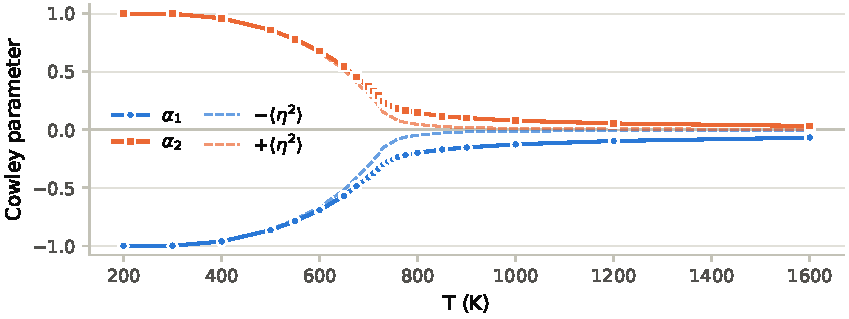
\includegraphics[width=0.9\textwidth]{cowley.pdf}

  \begin{itemize}
    \item Dashed: what long-range order alone gives ($\alpha_1=-\eta^2$, $\alpha_2=+\eta^2$)
    \item Above $\Tc$: $\eta\approx0$ but $\alpha_1<0$ $\Rightarrow$ Cu still prefers \alert{Zn neighbours}
  \end{itemize}
\end{frame}

% ---------------------------------------------------------------------
\begin{frame}{Transition temperature}
  \begin{columns}[c]
    \begin{column}{0.5\textwidth}
      \centering
      \begin{tabular}{lc}
        \toprule
        Method & $\Tc$ (K) \\
        \midrule
        Peak of $C$ & 720 \\
        Peak of $\chi$ & 720 \\
        Steepest drop of $|\eta|$ & 720 \\
        \midrule
        Mean field (Bragg--Williams) & 894 \\
        Experiment & $\approx 740$ \\
        \bottomrule
      \end{tabular}
    \end{column}
    \begin{column}{0.46\textwidth}
      \begin{itemize}
        \item Monte Carlo: \alert{close to experiment}
        \item Mean field~\cite{BraggWilliams1934}: $k_B\Tc = 2\,(E_\text{random} - E_\text{B2})$, \alert{170~K too high}
        \item Why? Mean field ignores short-range order, which stabilises the disordered phase
      \end{itemize}
    \end{column}
  \end{columns}
\end{frame}

% ---------------------------------------------------------------------
\begin{frame}{Limits and conclusion}
  \textbf{Limits}
  \begin{itemize}
    \item Small box (432 atoms): rounded transition, broad peaks
    \item Rigid lattice, pair energies: no vibrations, no size mismatch
    \item Near $\Tc$: slow, correlated sampling $\Rightarrow$ noisy $C$ and $\chi$
  \end{itemize}
  \textbf{Conclusion}
  \begin{itemize}
    \item Tested Metropolis code; cohesive energy \SI{2.484}{eV/atom}
    \item Order--disorder transition at \alert{$\Tc \approx \SI{720}{K}$} (experiment $\approx \SI{740}{K}$)
    \item Short-range order above $\Tc$ explains why mean field overestimates $\Tc$
    \item Next step: several box sizes to extrapolate $\Tc$ to an infinite crystal~\cite{LandauBinder2014}
  \end{itemize}
\end{frame}

% ---------------------------------------------------------------------
\begin{frame}[allowframebreaks]{References}
  \nocite{Sujet2026,BinderHeermann2019,Moss1964,KhanEisenbach2016}
  \printbibliography[heading=none]
\end{frame}

% ---------------------------------------------------------------------
\appendix
\begin{frame}{Backup: simulation conditions}
  \small
  \begin{tabular}{ll}
    \toprule
    Lattice & bcc, $6^3$ cells, 432 sites, periodic boundaries \\
    Start & perfect B2 at every temperature \\
    Moves & swap with a random first neighbour, Metropolis \\
    Equilibration & \num{50000} steps (116 sweeps), discarded \\
    Measurement & 4000 sweeps, one measurement per sweep \\
    Temperatures & 22 values, 200--1600 K, step 10 K near $\Tc$ \\
    Random numbers & Python \texttt{random} (Mersenne Twister), fixed seeds \\
    Cost & \SI{6.7}{\micro s} per step, 6 min for the whole study \\
    \bottomrule
  \end{tabular}
\end{frame}

\begin{frame}{Backup: why \texorpdfstring{$\alpha_1 = -\eta^2$}{alpha1 = -eta2} with long-range order only}
  \begin{itemize}
    \item Fraction of Cu on $\alpha$: $\frac{1+\eta}{2}$ \quad on $\beta$: $\frac{1-\eta}{2}$
    \item A Cu on $\alpha$ has its 1st neighbours on $\beta$, Zn with probability $\frac{1+\eta}{2}$
    \item A Cu on $\beta$ has its 1st neighbours on $\alpha$, Zn with probability $\frac{1-\eta}{2}$
    \[ p_1(\Zn|\Cu) = \left(\tfrac{1+\eta}{2}\right)^2 + \left(\tfrac{1-\eta}{2}\right)^2 = \frac{1+\eta^2}{2}
       \;\Rightarrow\; \alpha_1 = 1 - 2p_1 = -\eta^2 \]
    \item Same reasoning on the same sublattice: $\alpha_2 = +\eta^2$
  \end{itemize}
\end{frame}

\end{document}
